% !TEX encoding = UTF-8 Unicode
%!TEX root = ../Main/thesis.tex
% !TEX spellcheck = en-US
%%=========================================
\documentclass[../Main/thesis.tex]{subfiles}
\begin{document}
\chapter{Prototype Evaluation}
\label{ch:evaluation}
This chapter describes the final evaluation of the FireTracker system.
%The evaluation was done with representatives from Øygarden Fire and Rescue, at their offices and training facilities in Ågotnes.
The evaluation consisted of testing of the FireTracker system and evaluations using semi-structured interviews and SUS questionnaires.
The goal of this testing was to evaluate the FireTracker system in terms of usability for the fire department as a step in answering the research questions.

%\section{Preparations}
%As a preparation for the evaluation all the 14 available beacons were labeled with a number (See Figure~\ref{fig:beacons}) that matched the name they were given in the exercise management tool. 
%On the back side of the beacon another label was applied with the beacon's UUID, Major, and Minor values.
%The transmitting signal strength of all the beacons were set to the lowest possible value, and all of them were turned on.
%The two Android devices that was going to be attached to the smoke divers, and a backup device was fully charged.
%
%\begin{figure}[h]
%	\centering
%	\begin{subfigure}{0.8\textwidth}
%		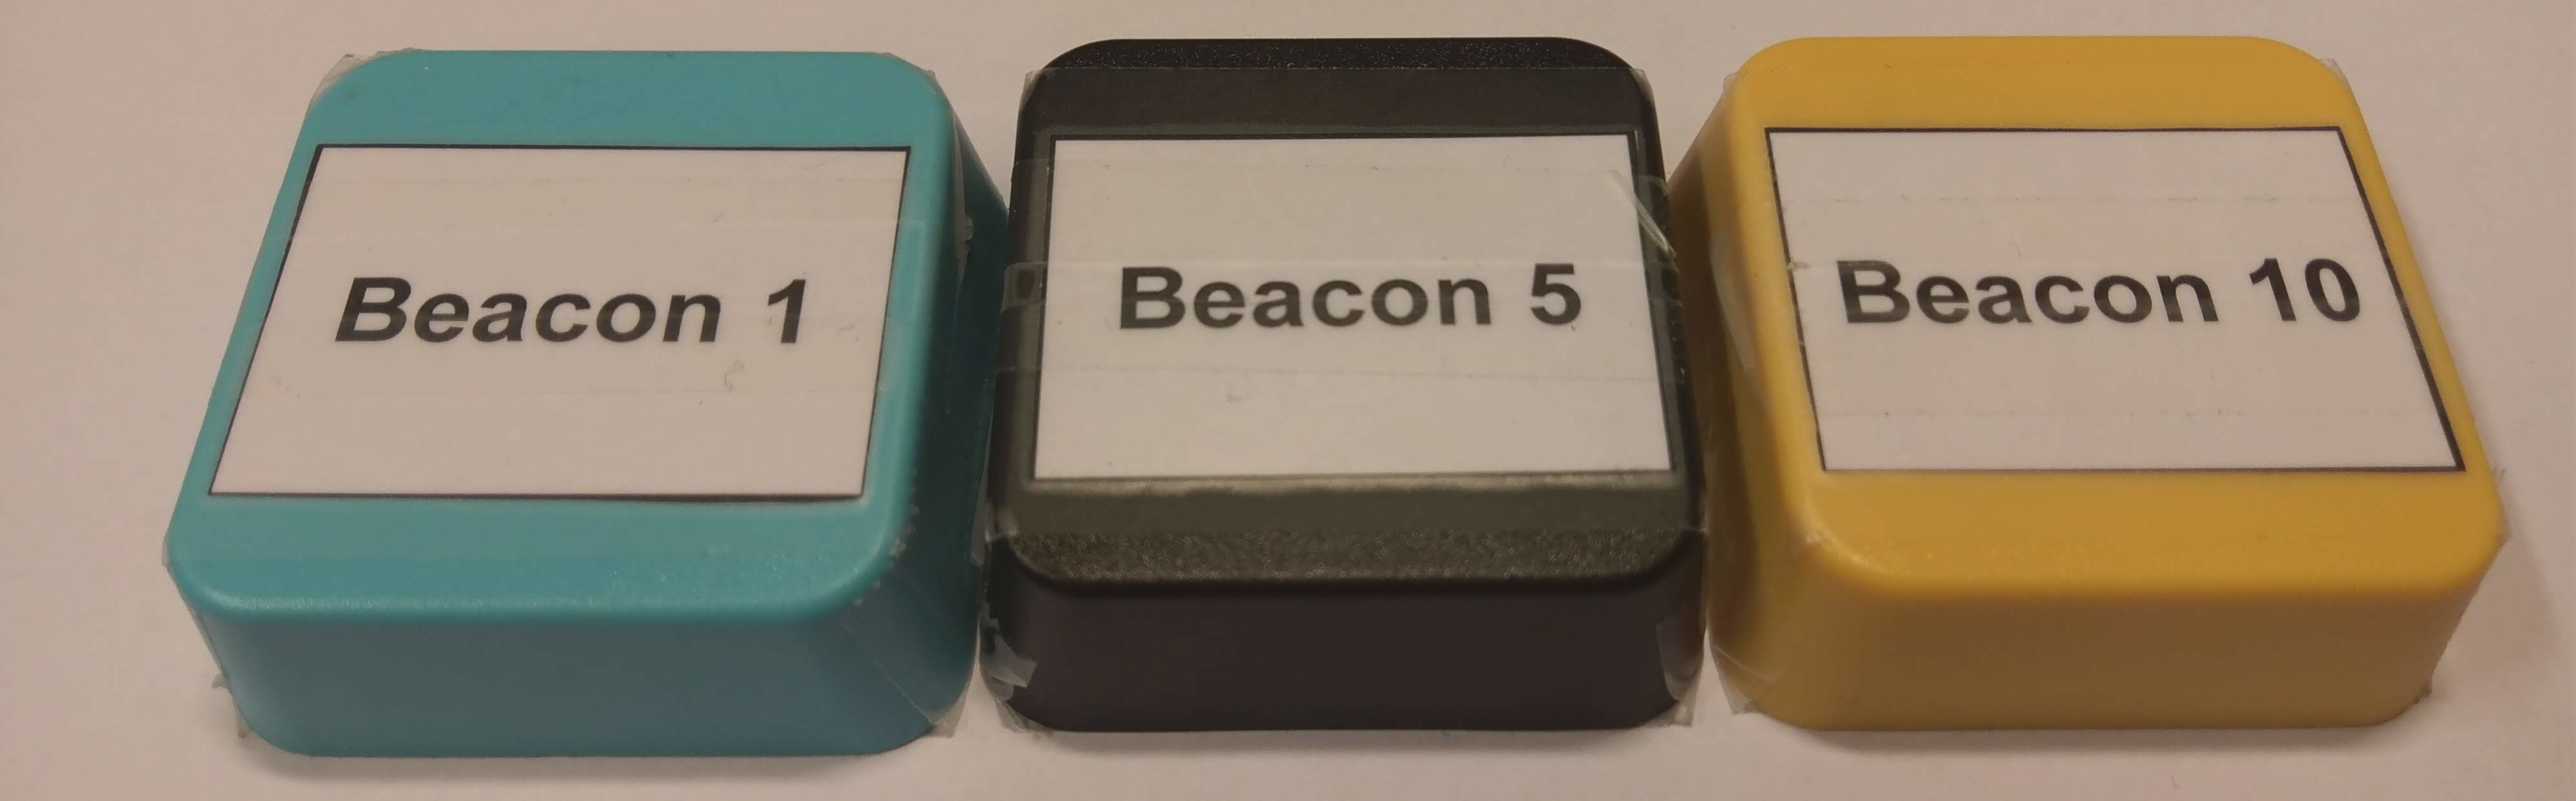
\includegraphics[width=\textwidth]{../fig/beacons-front}
%		\caption{Front of beacons}
%		\label{fig:beacons-front}
%	\end{subfigure}
%	\begin{subfigure}{0.8\textwidth}
%		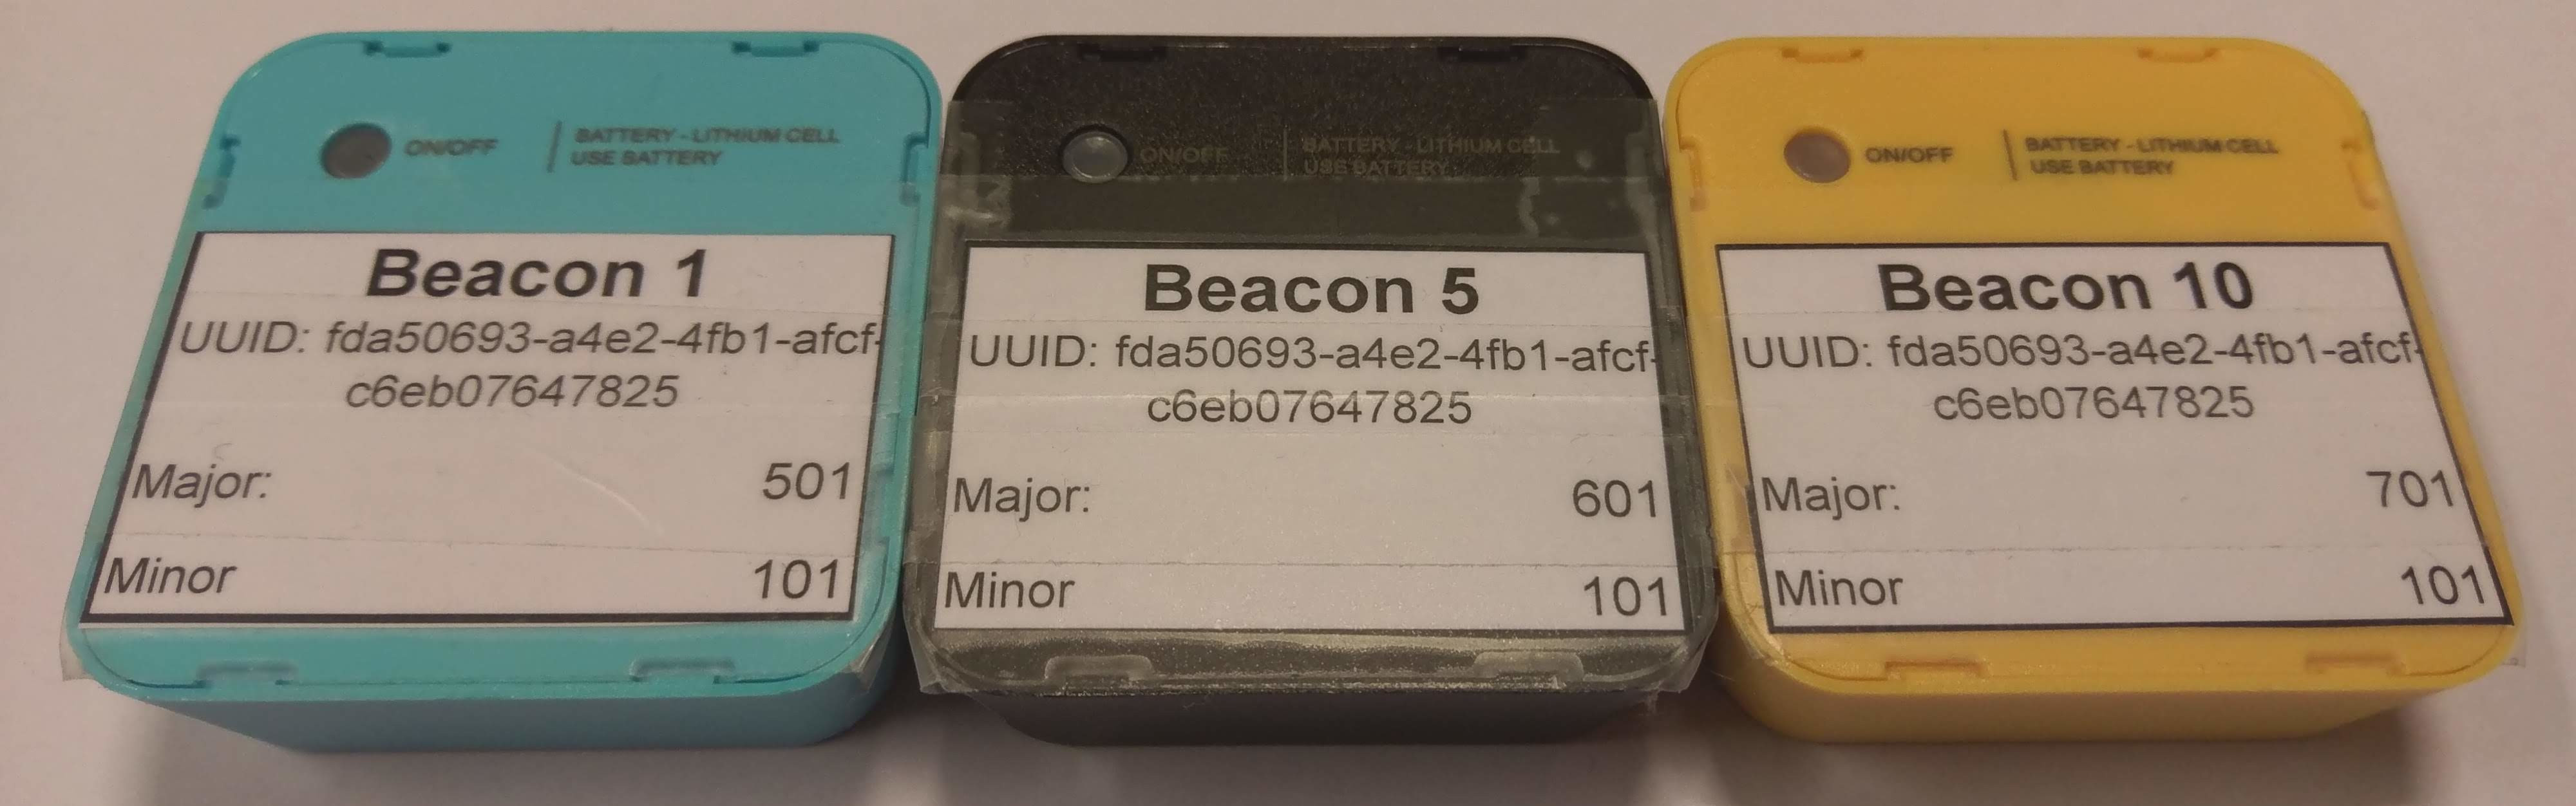
\includegraphics[width=\textwidth]{../fig/beacons-back}
%		\caption{Back of beacons}
%		\label{fig:beacons-back}
%	\end{subfigure}
%	\caption{Labeled BLE beacons}
%	\label{fig:beacons}
%\end{figure}

\section{Test of FireTracker}
The testing of the FireTracker system was done during a cold smoke exercise with Øygarden Fire and Rescue.

\subsection{Setting}
Figure~\ref{fig:eval-wireframe} shows the planned structure of the evaluation.
The first step in the evaluation was to present and introduce the project and system to all involved firefighters, both smoke divers, instructors, and other observers.
During this presentation both the exercise management tool and the Android application was demonstrated and explained, and questions from the firefighters regarding the use of the system was answered.
The location for the exercise was one of ØFR's empty, one floor, exercise buildings.
Before the exercise could start the building, beacons and sessions had to be set up.
As there was no floor plan available for the building one had to be drawn using pen and paper.
The instructors created a session in the exercise management tool, and placed beacons in areas they thought could be interesting.

\begin{figure}[h]
	\centering
	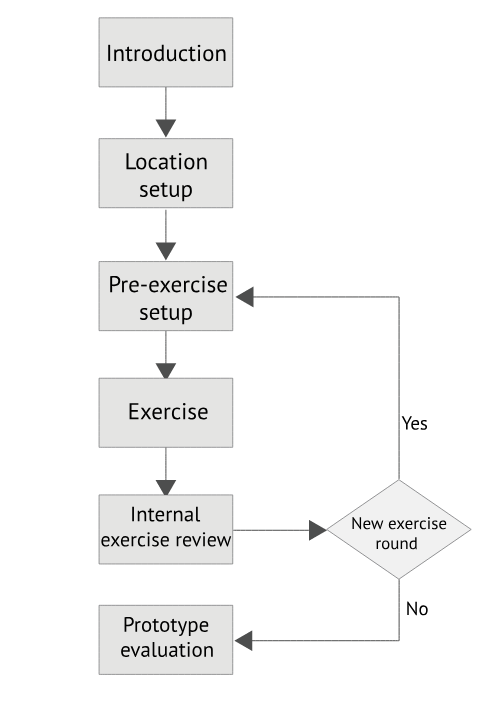
\includegraphics[width=0.4\textwidth]{../fig/eval_wireframe}
	\caption{Wireframe of evaluation}
	\label{fig:eval-wireframe}
\end{figure}

When the beacons were placed in the building, and other necessary equipment, such as the smoke machine, was in place the mobile phones was set up with the correct sessions for each smoke diver, the tracking was activated and the phones were placed in a container attached to the smoke diver's helmet as shown in Figure~\ref{fig:eval-helmet}.

\begin{figure}[h]
	\centering
	\begin{subfigure}{0.22\textwidth}
		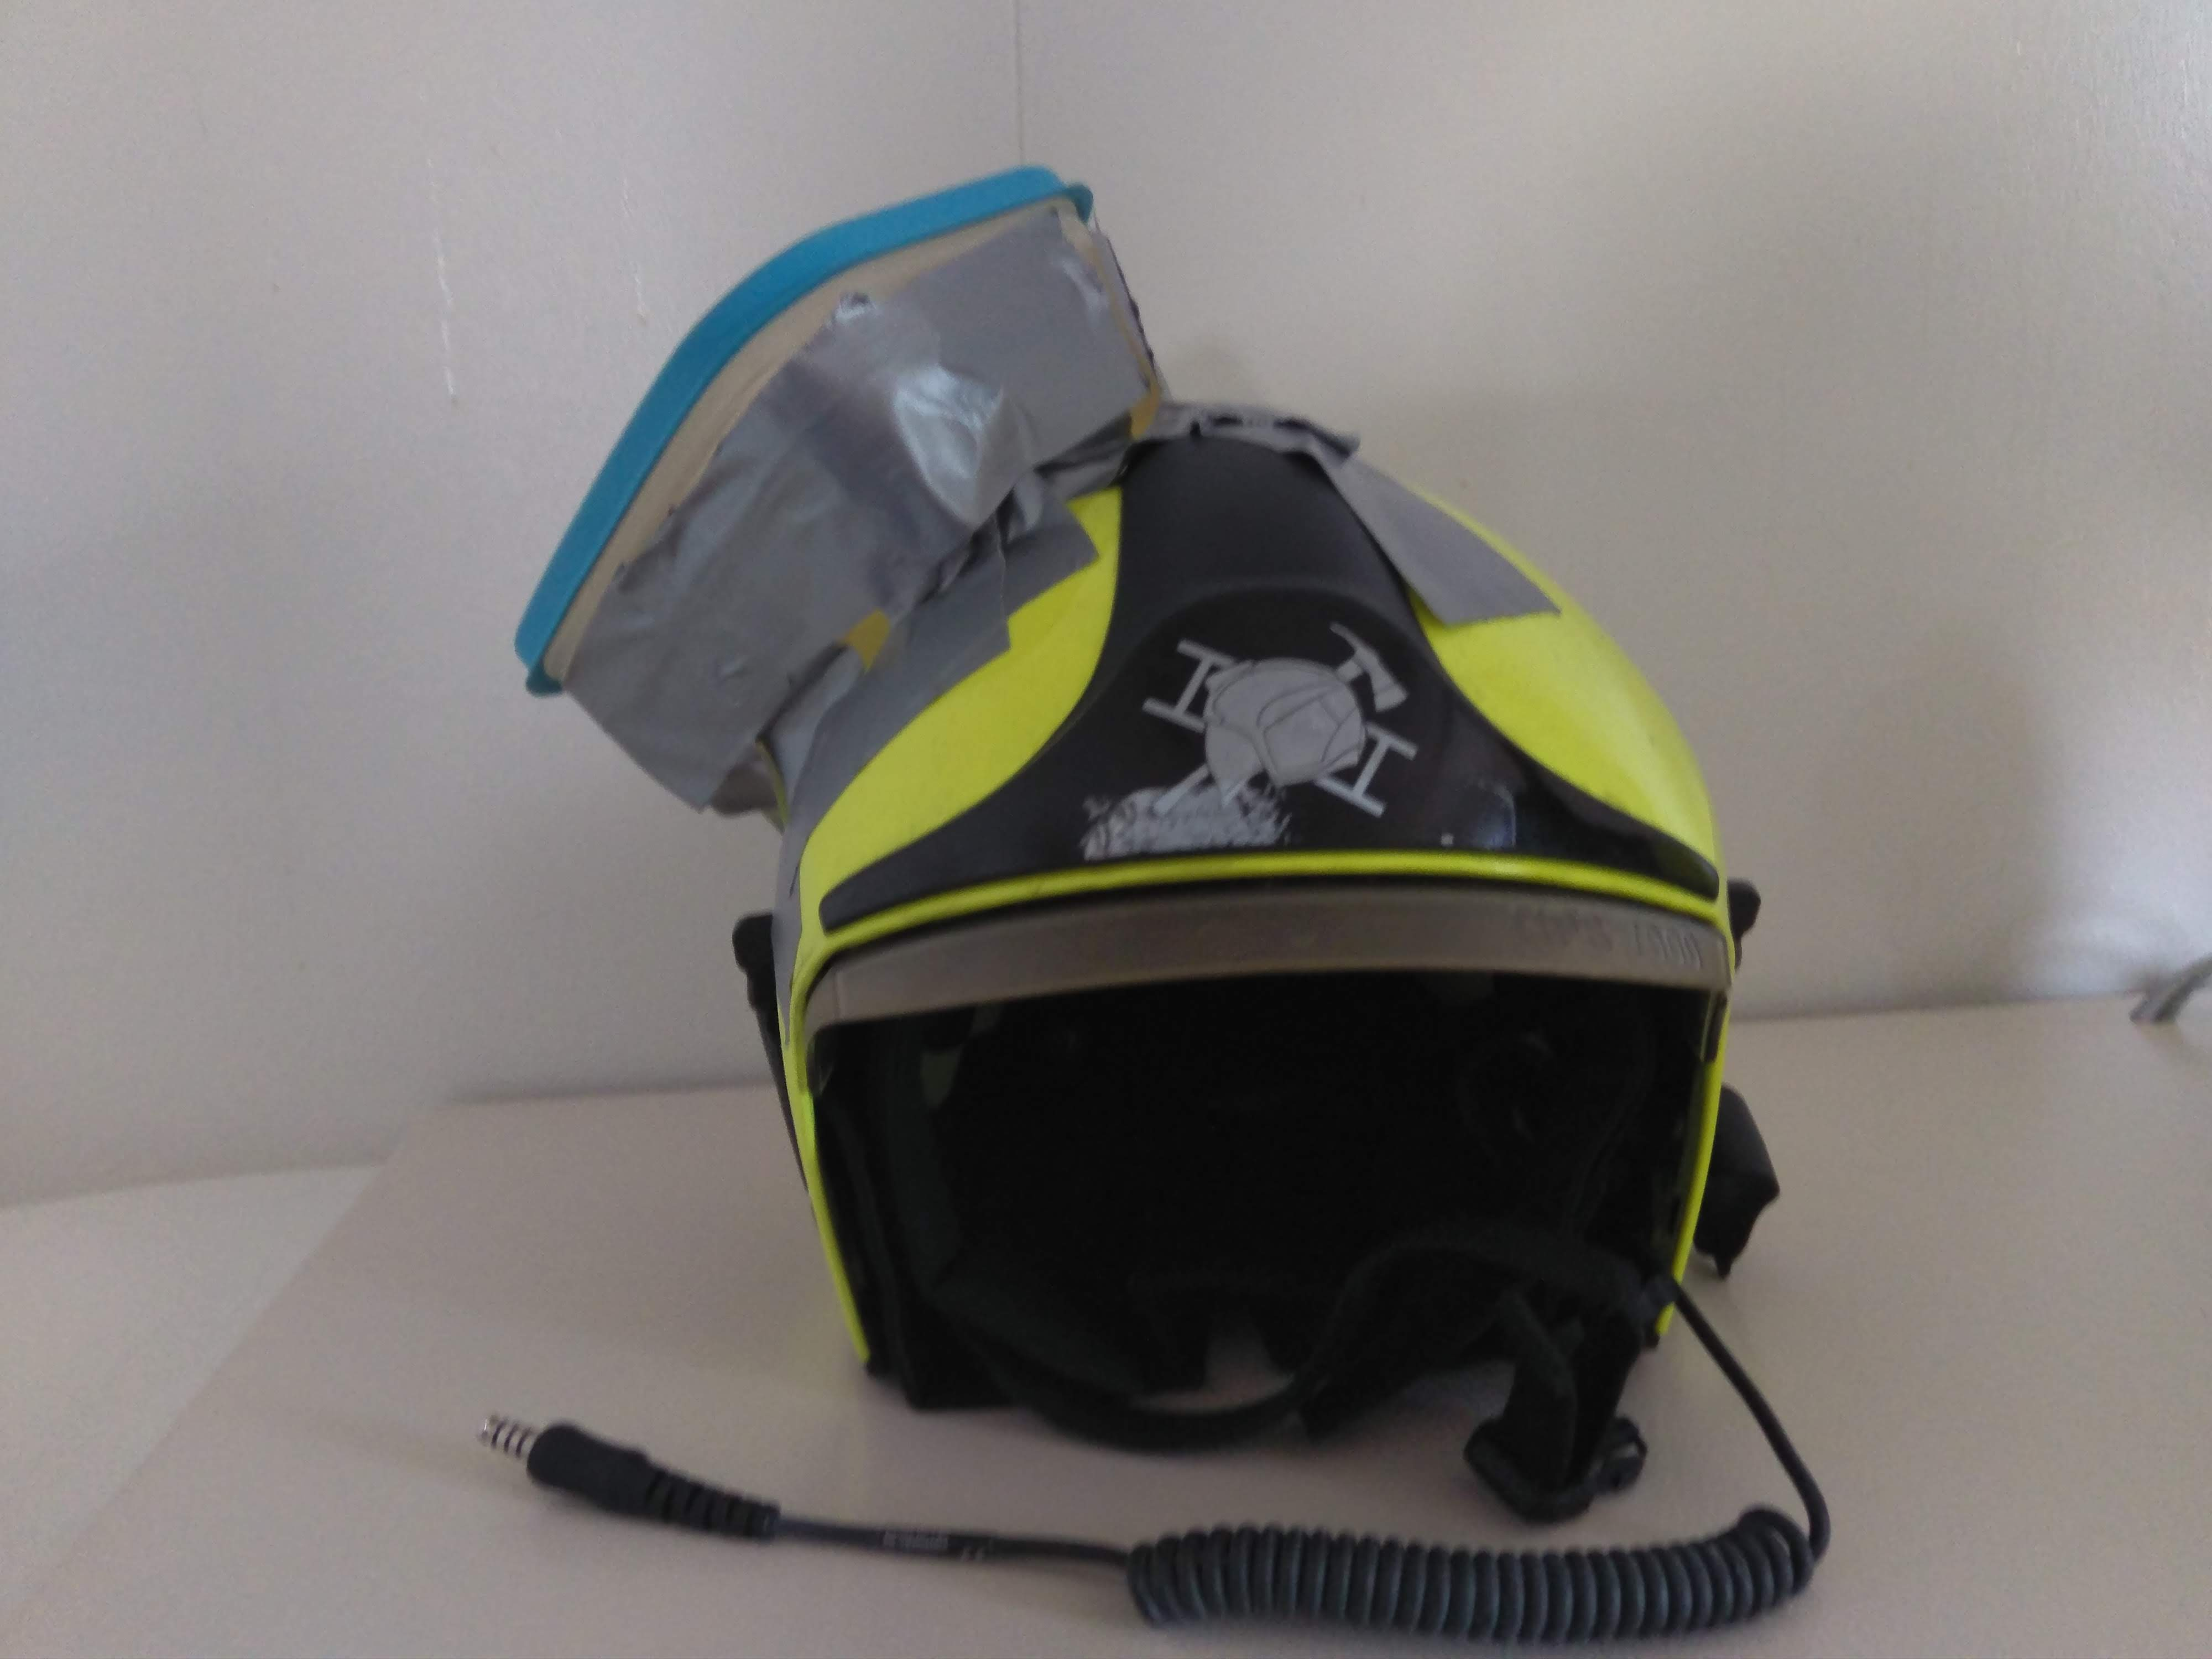
\includegraphics[width=\textwidth]{../fig/helmet-front}
		\caption{Front of helmet}
		\label{fig:eval-helmet-front}
	\end{subfigure}
	\begin{subfigure}{0.22\textwidth}
		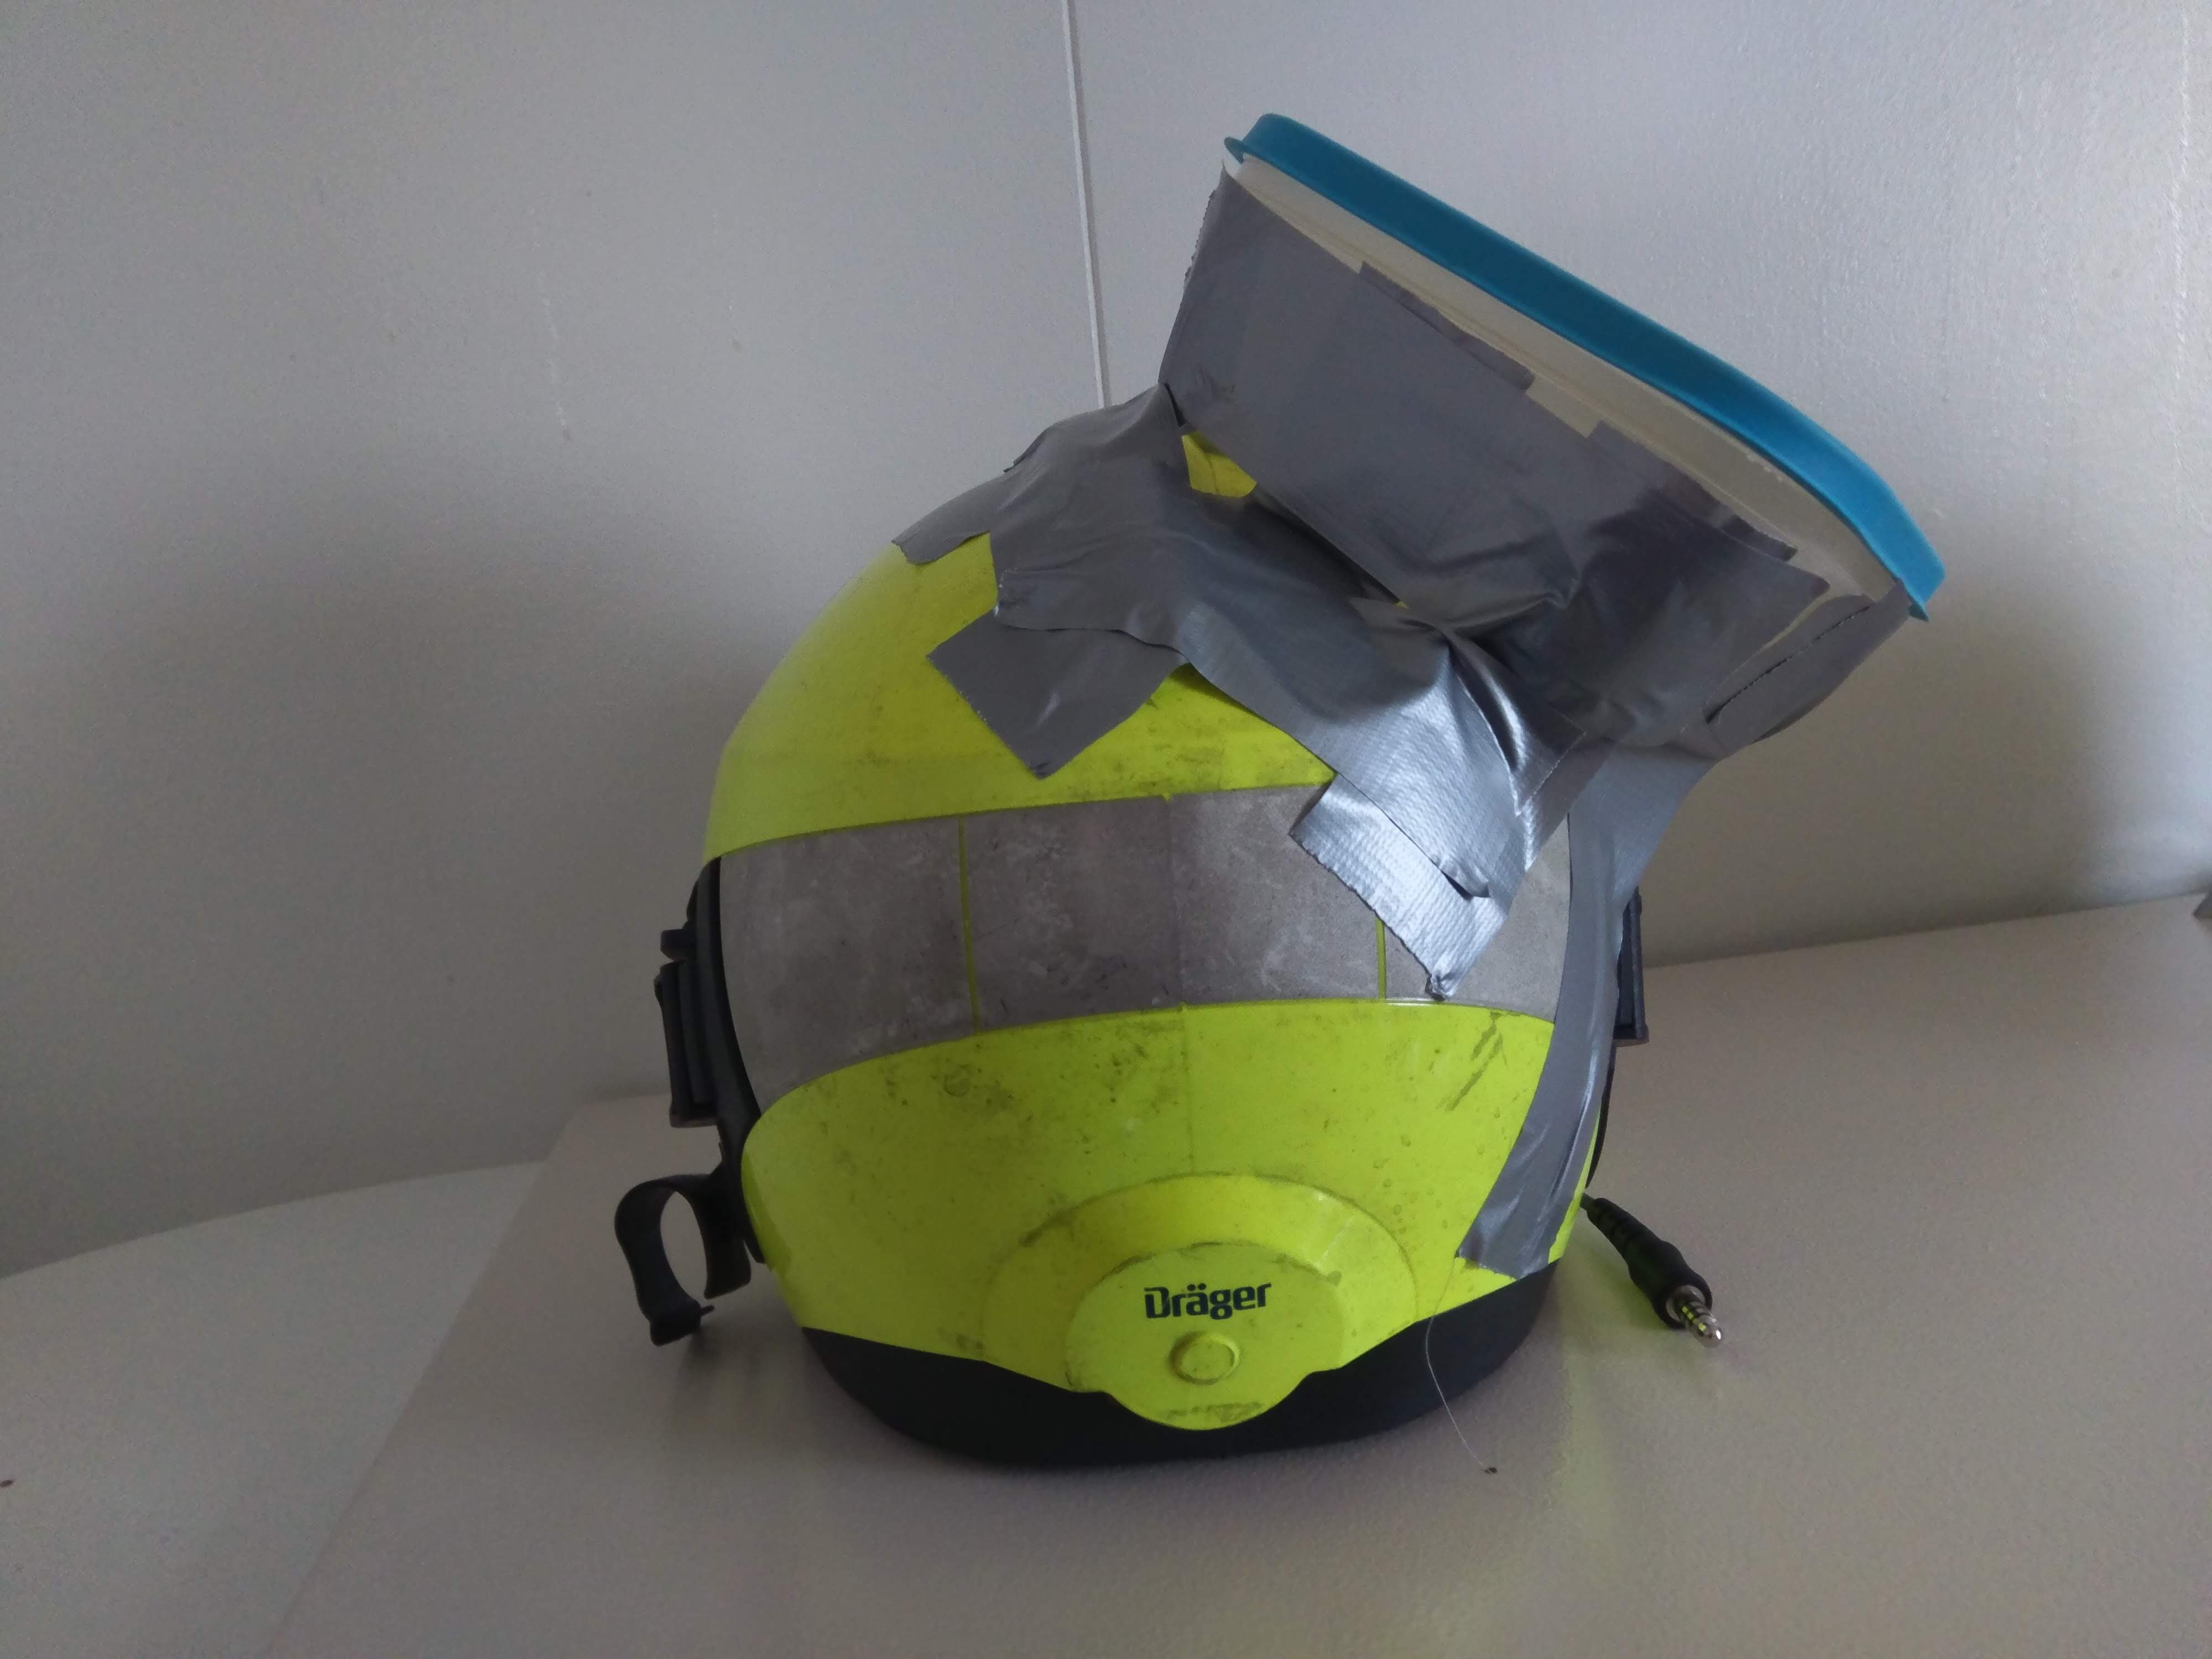
\includegraphics[width=\textwidth]{../fig/helmet-back}
		\caption{Backside of helmet}
		\label{fig:eval-helmet-back}
	\end{subfigure}
	\begin{subfigure}{0.22\textwidth}
		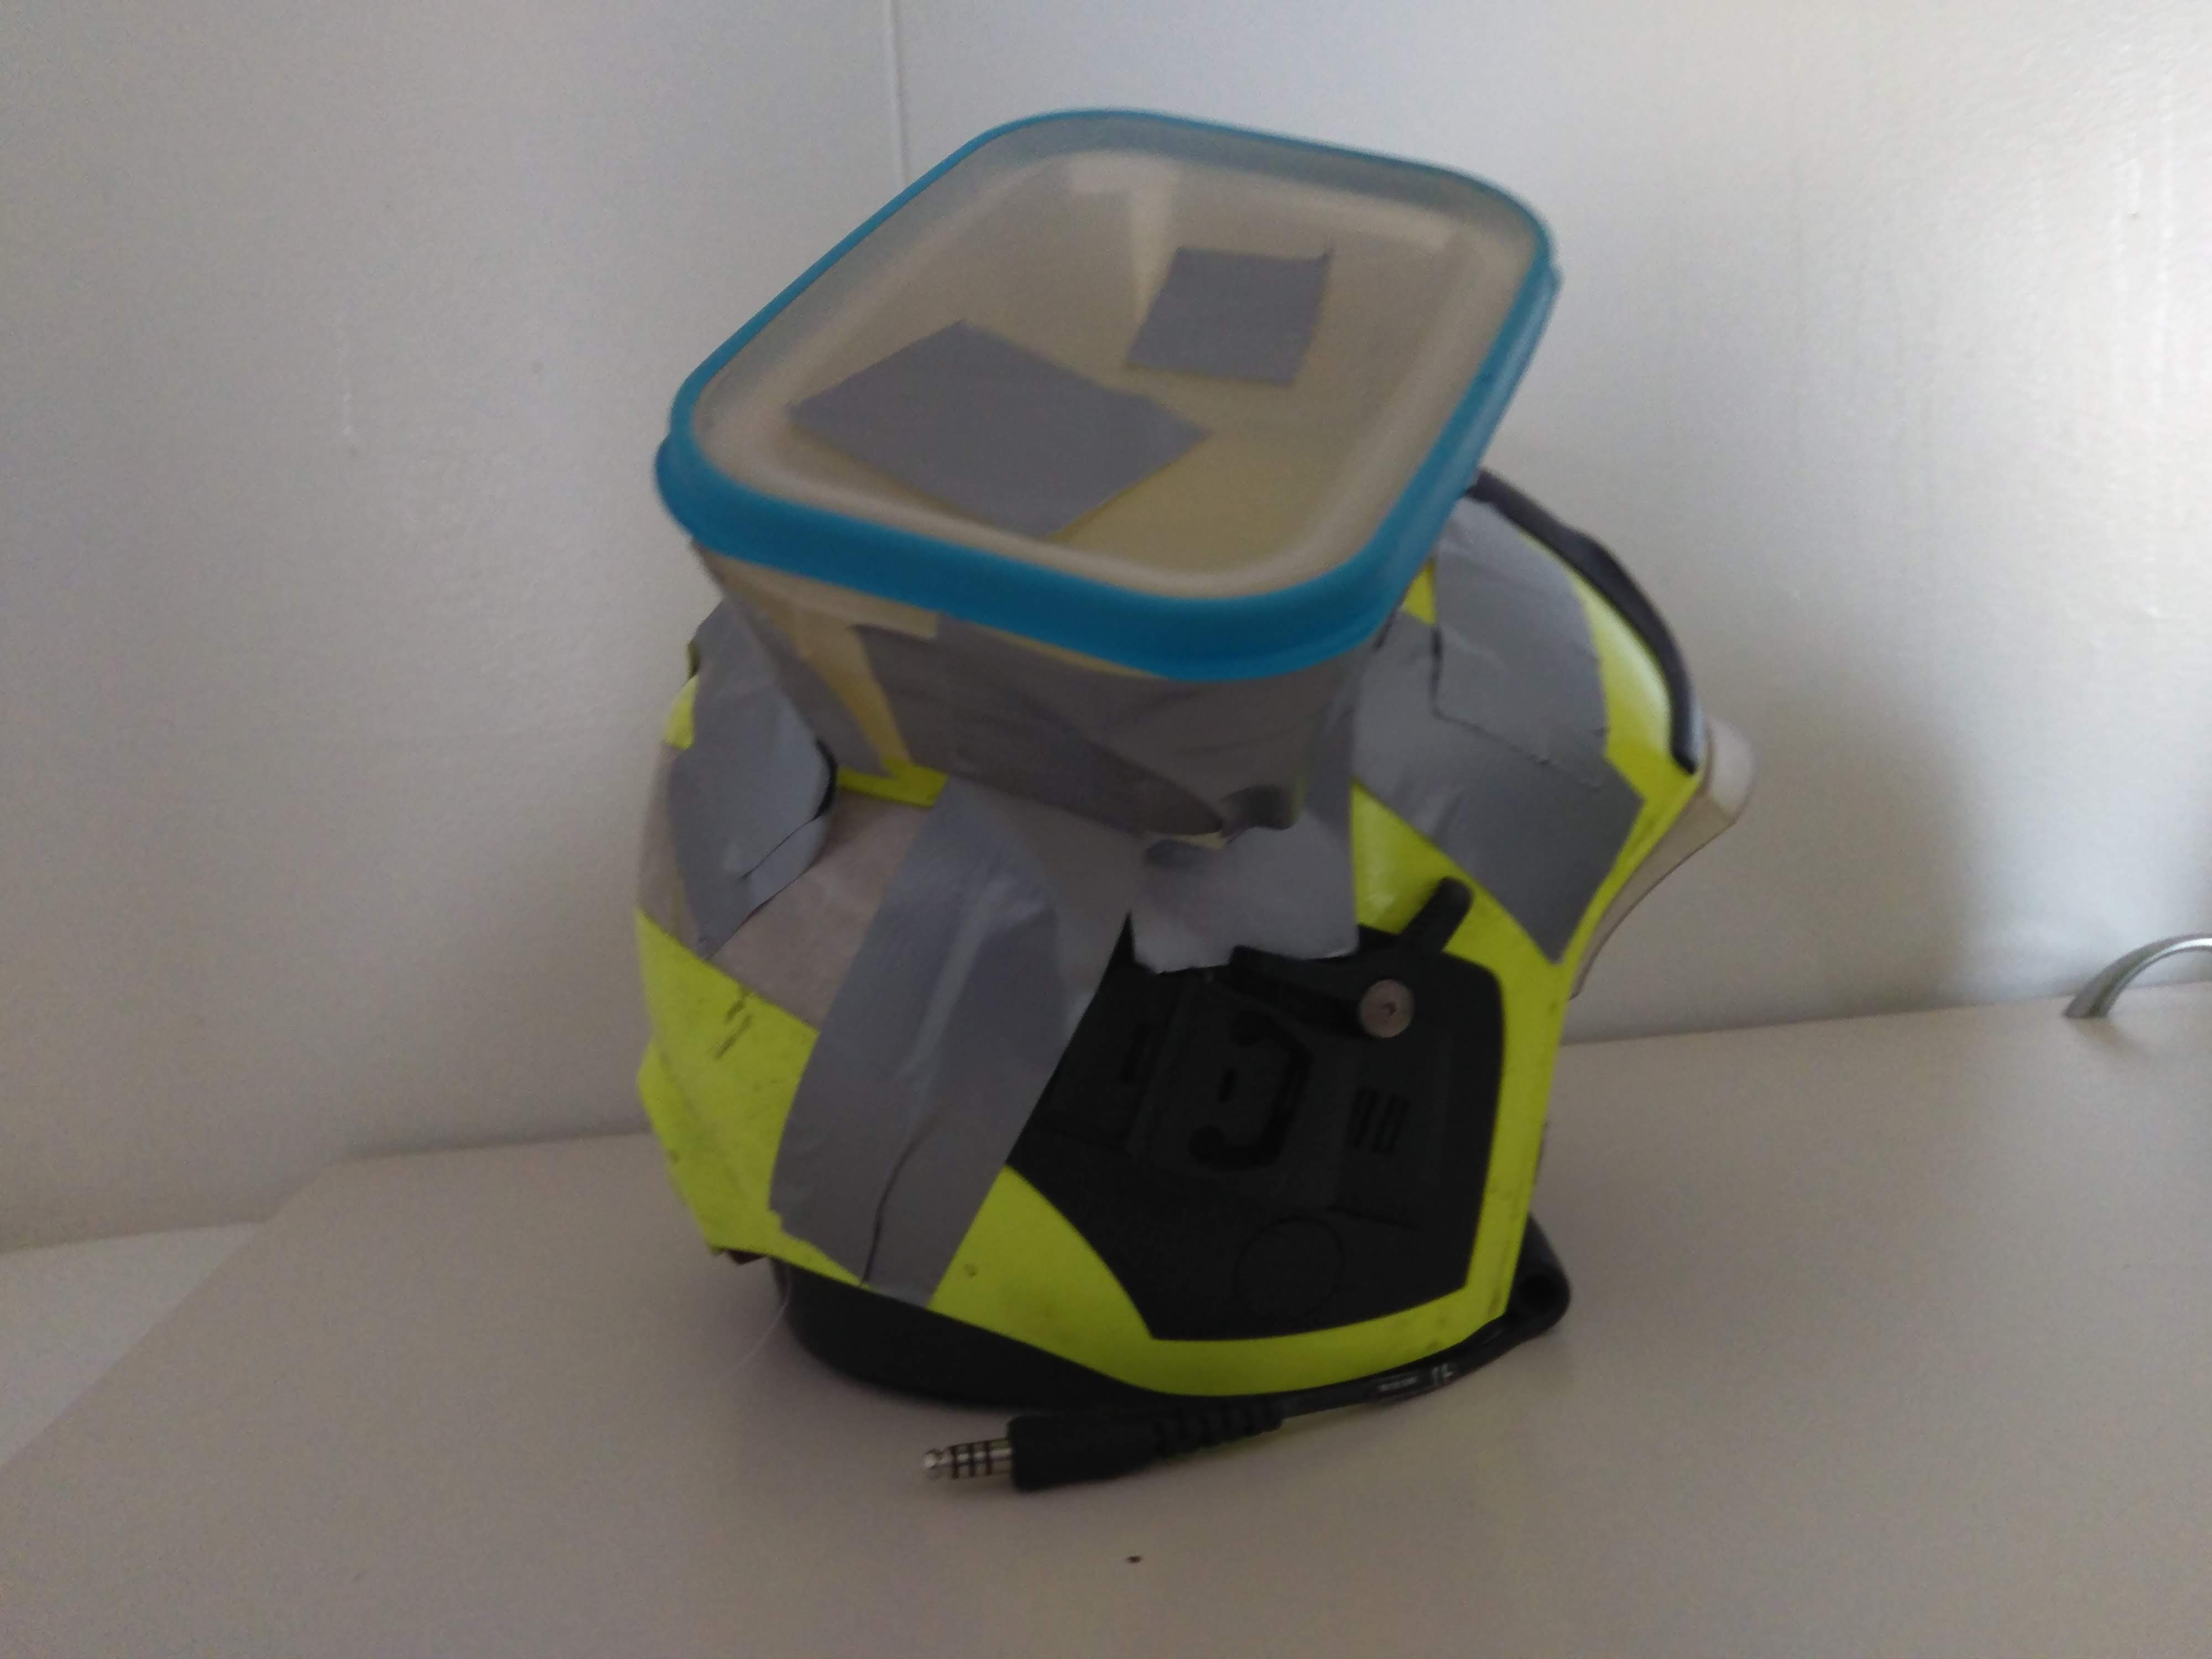
\includegraphics[width=\textwidth]{../fig/helmet-right}
		\caption{Right side of helmet}
		\label{fig:eval-helmet-right}
	\end{subfigure}
	\begin{subfigure}{0.22\textwidth}
		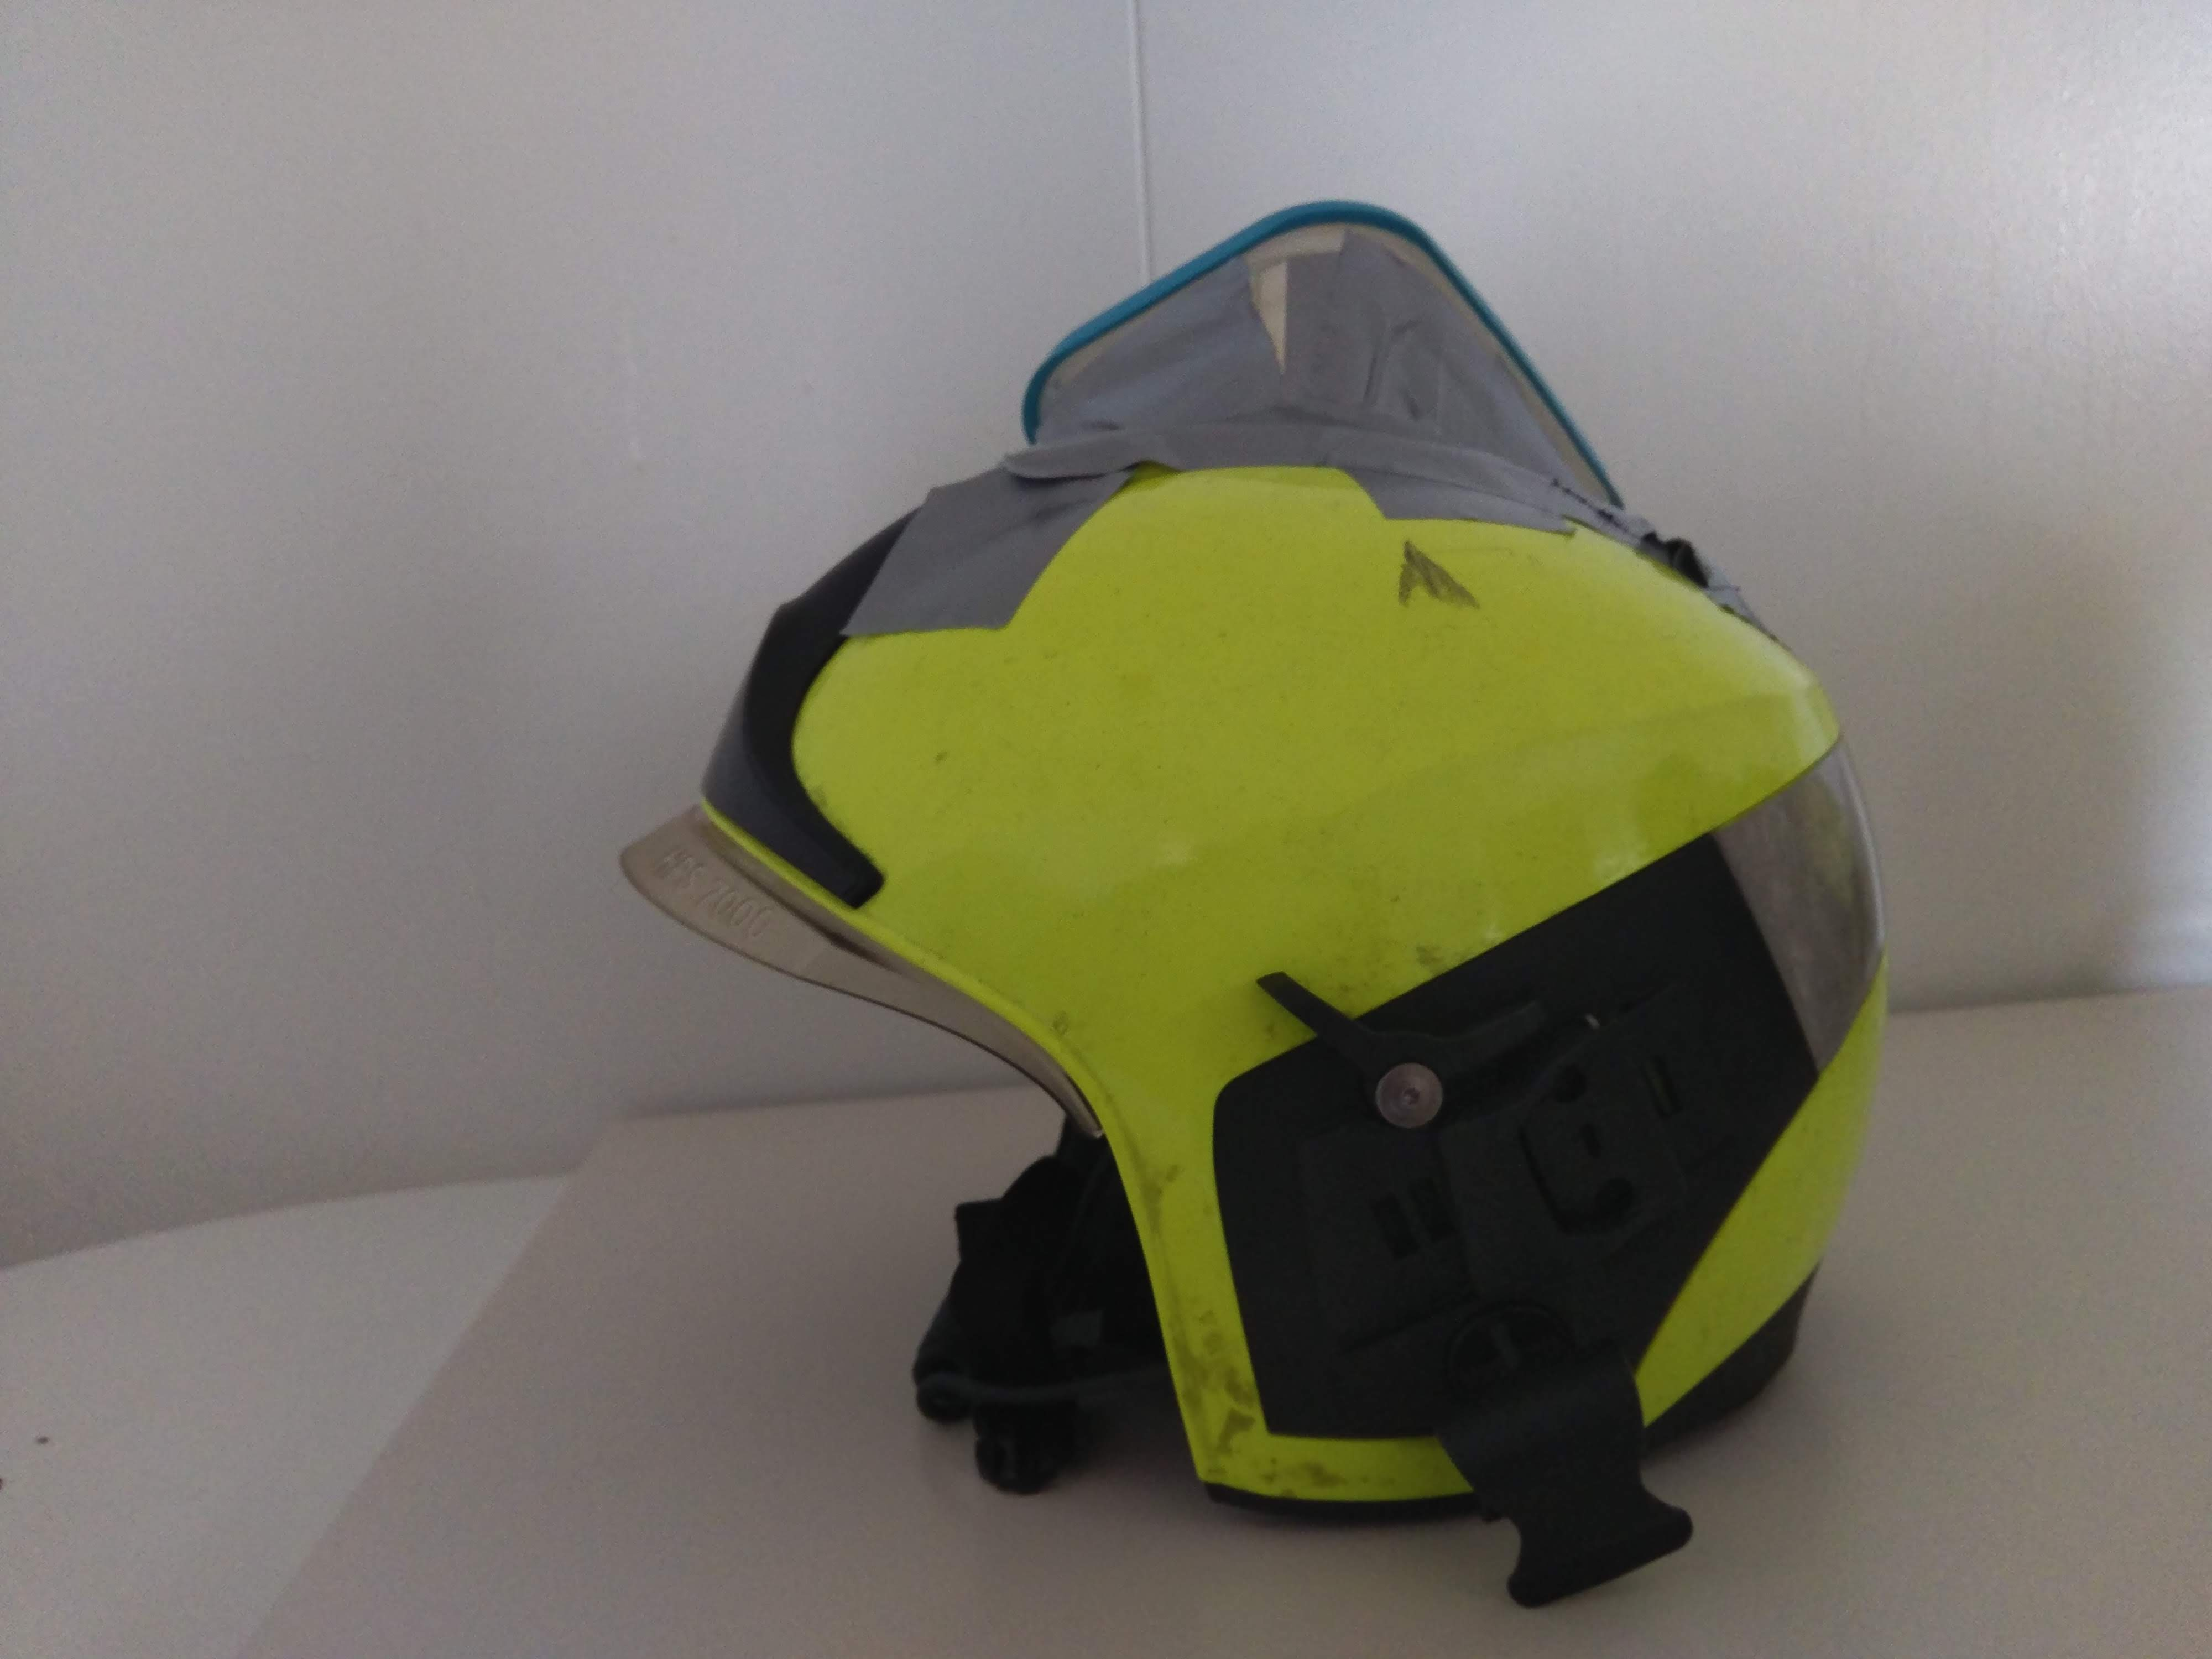
\includegraphics[width=\textwidth]{../fig/helmet-left}
		\caption{Left side of helmet}
		\label{fig:eval-helmet-left}
	\end{subfigure}
	\caption{Plastic box for smartphone attached to helmet}
	\label{fig:eval-helmet}
\end{figure}

\subsection{Participants}
Øygarden Fire and Rescue provided four firefighters for the evaluation.
Two of them were smoke divers and two of them were instructors.
The instructors also played the roles as smoke diver leader, fire chief, and firefighter squad leader.
The smoke divers has two roles: smoke diver 1 and smoke diver 2.
Smoke diver 1's role is to lead the work, use the fire hose, and search the area \citep{Direktoratetforsamfunnssikkerhetogberedskap1994}. /todo{Fiks referanse}
Smoke diver 2's role is to feed the fire hose to smoke diver 1, carry equipment, open doors, and search the area.% \citep{Direktoratetforsamfunnssikkerhetogberedskap1994}.
The smoke diver leaders role is to maintain contact with the smoke divers, keep track of time and oxygen levels of the smoke divers, be ready to enter the building in case of an emergency, and feed fire hose to the smoke divers.

\subsection{Data Collection}
The exercises were observed by the researches who also took notes and pictures during the sessions. 
The first session was done without smoke, instead the smoke divers' masks were covered with plastic bags, which allowed the researchers to observe from inside the building

\subsection{Flow of Exercise}
There were four smoke diving sessions.
The first three of them were performed with full smoke diving gear, as in a real-life situation, and the last was performed without gear.

\textbf{Setup of each smoke dive:}
\begin{enumerate}
	\item Two smoke divers and one instructor. No smoke in the building, but the smoke divers' mask was covered in plastic.
	\item Two smoke divers and one instructor. Building filled with smoke.
	\item Two smoke divers and one instructor. Building filled with smoke.
	\item One smoke diver and one instructor. No smoke in building.
\end{enumerate}

As the smoke divers masks were covered in the fist session their visibility was zero and they had to rely on their other senses.
For the second and third session the building was covered in cold smoke, which give the smoke divers some visibility.
The last session was done without gear and smoke to present some more data were the actions of the smoke divers were observable.
After each session the collected data from the Android application was uploaded and the visualizations was presented to the smoke divers and instructors who discussed them.
Figure~\ref{fig:eval-firefighters} shows the smoke divers discussing search strategy with the instructor before entering the building.

\begin{figure}[h]
	\centering
	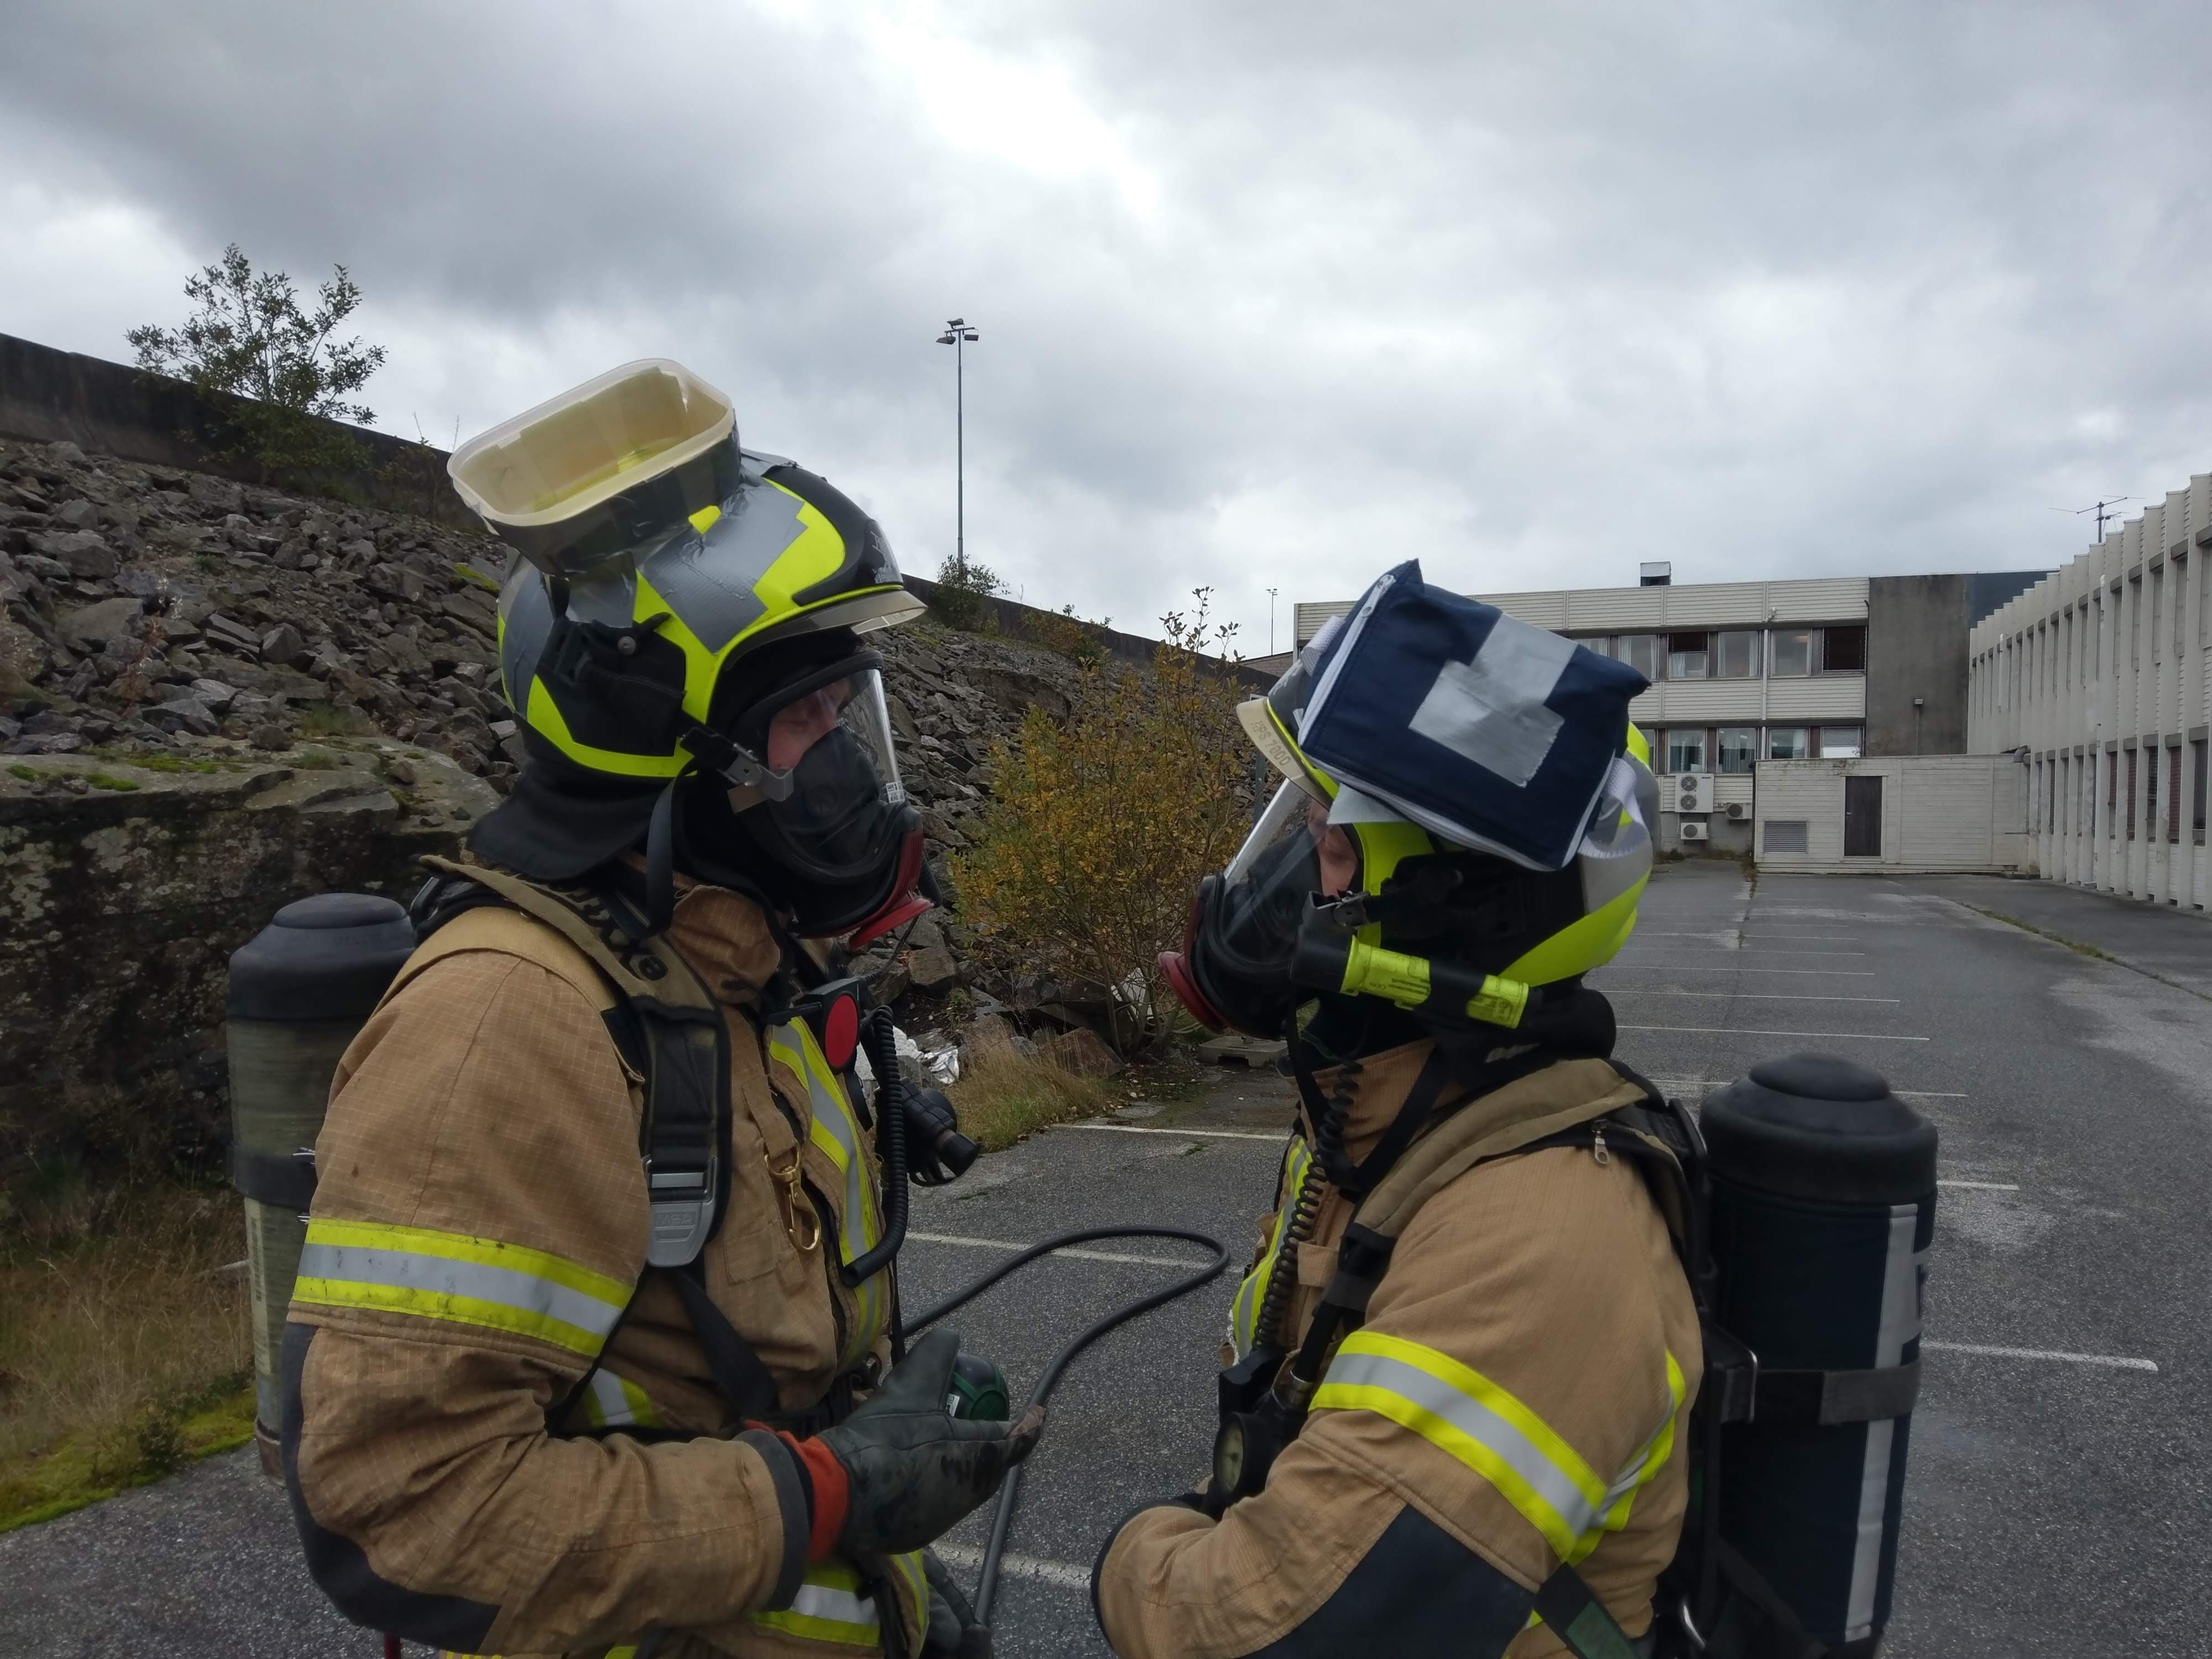
\includegraphics[width=\textwidth]{../fig/firefighters-with-helmet}
	\caption{Firefighters with smartphones mounted on their helmet}
	\label{fig:eval-firefighters}
\end{figure}

\subsection{Analysis}
In the first exercise five beacons were used, with one in each corner of the building and one approximately in the center as shown in Figure~\ref{fig:visualization-1-1}.
This visualization gives a somewhat accurate overview of the smoke divers movement, but there are some lines that do not match the actual movements.
This inaccuracy exists because the Android application registers signals from several beacons at the same time, and cannot decide the exact position, as explained in Chapter~\ref{sec:iteration3-testing}

\begin{figure}[h]
	\centering
	\begin{subfigure}{0.3\textwidth}
		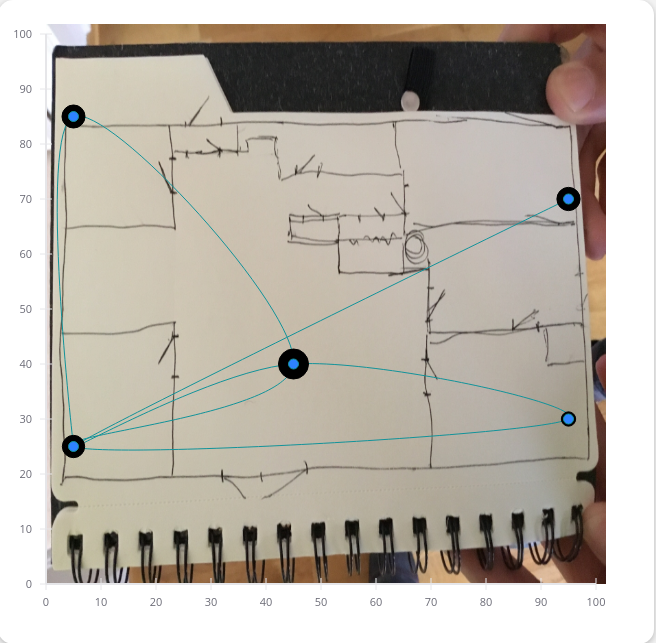
\includegraphics[width=\textwidth]{../fig/eval_1_remi}
		\caption{Exercise 1, smoke diver 1}
		\label{fig:visualization-1-1}
	\end{subfigure}
	\begin{subfigure}{0.3\textwidth}
		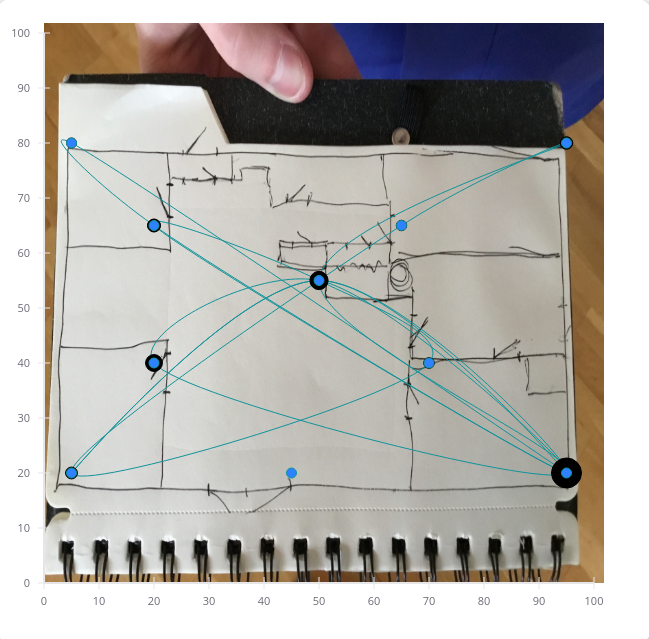
\includegraphics[width=\textwidth]{../fig/eval_2_remi}
		\caption{Exercise 2, smoke diver 1}
		\label{fig:visualization-2-1}
	\end{subfigure}
	\begin{subfigure}{0.3\textwidth}
		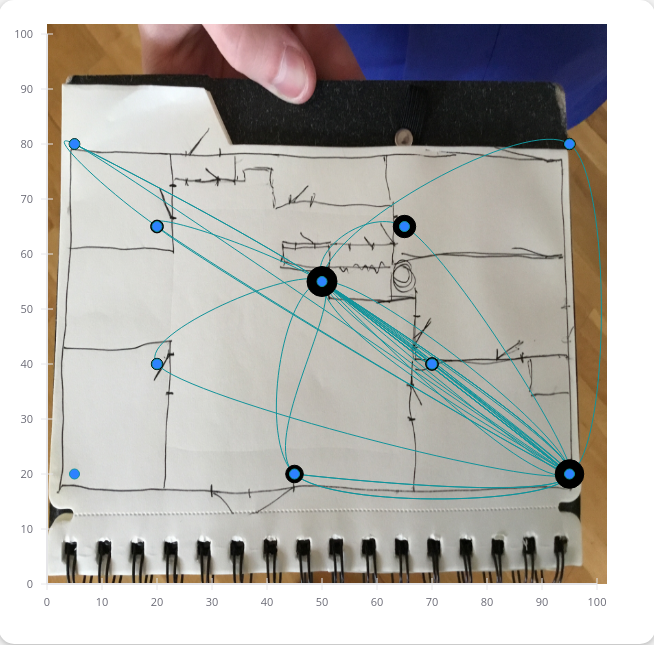
\includegraphics[width=\textwidth]{../fig/eval_2_fredrik}
		\caption{Exercise 2, smoke diver 2}
		\label{fig:visualization-2-2}
	\end{subfigure}
	\caption{Visualizations for exercise 1 and 2}
	\label{fig:eval-visualizations}
\end{figure}

In the later exercises the number of beacons used are increased, as shown in Figure~\ref{fig:visualization-2-1} and Figure{fig:visualization-2-2}.
This was done to test if having multiple beacons in the same room would give a better tracking and information about the search technique.
In this case the effect of the too strong signal strength is even clearer, but there is also a difference in the number of lines on the visualization for smoke diver 1 (Figure~\ref{fig:visualization-2-1}) and smoke diver 2 (Figure~\ref{fig:visualization-2-1}), where smoke diver 2 has much more lines.
This could be an indication on a higher level of activity on smoke diver 2, which fits well with their tasks, as smoke diver 2 is supposed to move more around.
It also matches what the smoke divers themselves told about their activity level.

The third and fourth exercise shows similar results as exercise 2.
There is much noise in the visualizations because the Android app detects beacons that are not nearby.
A difference in activity level can also be seen in those visualizations, and they those exercises as well they correspond to the smoke divers roles and reported activity.
The visualizations for these exercises can be found in Appendix~\ref{app:visualizations}.

\section{Evaluation}
After the testing there was an evaluation session.
The evaluation was performed as a semi-structured interview with each of the participants followed by a SUS questionnaire.
The interviews were recorded and transcribed.
Interview guides can be found in Appendix~\ref{app:interview-guide-final}
The SUS questionnaire can be found in Appendix~\ref{app:sus}.

\subsection{Evaluation with smoke divers}
The smoke divers were asked questions about how the use of FireTracker affected their performance.
Their answers was that it had no impact on how they behaved, because they were so focused on their tasks that they forgot they had the phones on their helmet.
They also said that using a few seconds to start the tracking before entering the building did not matter in this setting, but in the future it should already attached to their bodies before arriving the location, and they already have other equipment that is attached and activated in the car en route to the exercise.

They were also asked about how the system could be used during their evaluation of an exercise.
To this they answered that the current version of the visualizations are too cluttered with all the incorrect lines, but they think the system has potential to become useful.
They also stated that they wanted a higher level of precision on the tracking.
Instead of all points and lines showing up at once, they would prefer to have the graph drawn as they step through each visited location.

Figure~\ref{fig:sus-smoke-divers} shows the smoke divers' scores on the SUS questionnaire.
Both of the smoke divers scored below 68, which is the lower limit for what \citet{Brooke2013} considers a good score.

\begin{figure}[h]
	\centering
	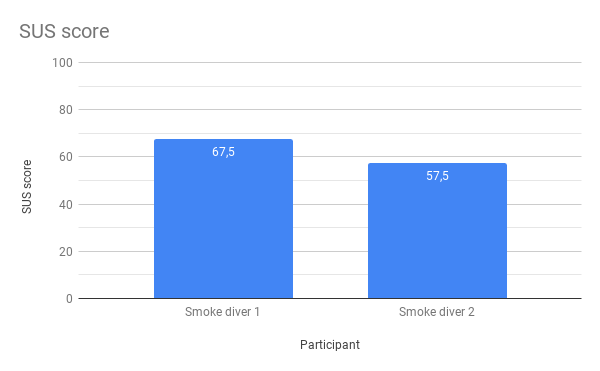
\includegraphics[width=\textwidth]{../fig/sus-smoke-divers.png}
	\caption{SUS score for the smoke divers}
	\label{fig:sus-smoke-divers}
\end{figure}

\subsection{Evaluation with instructors}
The instructors were asked questions about how it was to use the system, both about the user interface, and the physical setup and use.
Both instructors agreed that the system was easy set up and use.
They thought it was user friendly and easy to understand.
One of them also said that if they were to use FireTracker in real exercises they would attach and activate the tracking devices before they left the fire station or in the car on the way to the exercise location, as they do with other equipment.
It was also mentioned that the helmet might not be the ideal placement of the phones, as it is a very exposed position.

\begin{figure}[h]
	\centering
	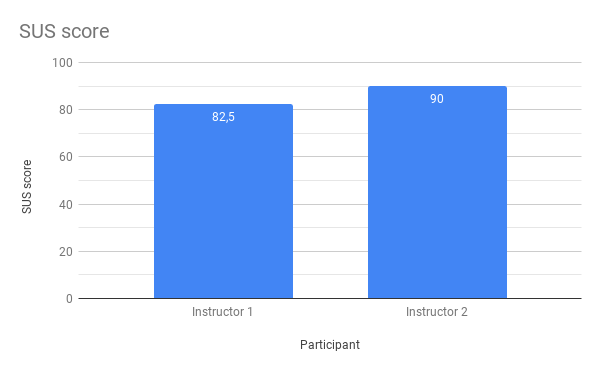
\includegraphics[width=\textwidth]{../fig/sus-instructors.png}
	\caption{SUS score for the instructors}
	\label{fig:sus-instructors}
\end{figure}

They were also asked about the data the system provided, and how they contributed to the exercise evaluation.
Both of the instructors thought the data collected was relevant, but in the current version the data was not good enough because it showed the user as being somewhere else than they actually were at times.
They were also positive to the visualization of time usage, as it can show if a smoke diver hesitates somewhere he should not be hesitating, or at what part of the exercise a smoke diver spends most time.
This can be used in their discussions after the exercise, and it could be used to understand what the individual smoke divers need to exercise more of in the future.
One of them also said that it could be interesting to combine the tracking with video footage from a camera attached to the smoke diver.
It was suggested to use beacons with a very short range to track if a specific object, such as a bed, had been searched.

Figure~\ref{fig:sus-instructors} shows the instructors' scores on the SUS questionnaire.
Both of the instructors scored above 68, which is the limit for what is considered a good score \citep{Brooke2013}.


\section{Summary}
This chapter described the evaluation of the FireTracker system that was performed as a test in a real-life cold smoke diving exercise with Øygarden Fire and Rescue, and followed up by interviews and SUS questionnaires.


\end{document}
